%% Genatic Algorthims introduction
%%%%%%%%%%%%%%%%%%%%%%%%%%%%%%%%%%%%%%%%%%%%%%%%%%%%%%%%%%%%%%%%%%%%%%%%%%
\begin{frame}{Genetic Algorithms}
A search technique mimicking natural evolution.
\begin{columns}[onlytextwidth]
  \begin{column}{0.45\textwidth}
    \small
    \begin{itemize}
      \item Population of candidate solutions is evolved toward better solutions
      \item Each candidate has properties that can be mutated and altered
      \item Traditionally solutions are represented as bit strings or trees
    \end{itemize}
    \end{column}
  \begin{column}{0.45\textwidth}
    \begin{figure}
		\tiny
		\begin{algorithmic}
      \WHILE{$error>goal$}
        \FORALL{$p \in P$}
          \STATE{Compute fitness}
        \ENDFOR
        \FORALL{$p \in P$}	
          \STATE{Choose individuals based on fitness}
          \STATE{Select individuals for next population}
          \STATE{Crossover selected individuals}
          \STATE{Mutate selected individual}
        \ENDFOR
      \ENDWHILE
    \end{algorithmic}
    \end{figure}
  \end{column}
\end{columns}
\hyperlink{GAMethod}{\beamerbutton{Return to Optimization}}
\hyperlink{toc}{\beamerbutton{Table of Contents}}
\end{frame}
%%%%%%%%%%%%%%%%%%%%%%%%%%%%%%%%%%%%%%%%%%%%%%%%%%%%%%%%%%%%%%%%%%%%%%%%%%
\begin{frame}{Crossover Operations}
	\begin{columns}[onlytextwidth]
	\begin{column}{0.4\textwidth}
  \begin{itemize}
    \item Single point - choose a single point (two segments) to crossover
    \item Two point - choose two points (three segments) to crossover
    \item Uniform - Uniformly cross over based on some probability
  \end{itemize}
	\end{column}
	\begin{column}{0.55\textwidth}
    \begin{figure}
      \centering
      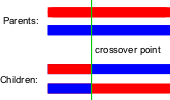
\includegraphics[width=0.3\textwidth]{SinglePointCrossover.png}
    \end{figure}
    \begin{figure}
      \centering
      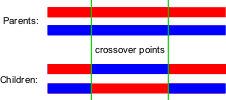
\includegraphics[width=0.3\textwidth]{TwoPointCrossover.png}
    \end{figure}
    \begin{figure}
      \centering
      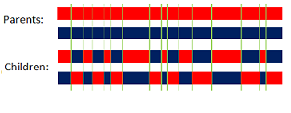
\includegraphics[width=\textwidth]{UniformCrossover.png}
    \end{figure}
	\end{column}
	\end{columns}
\hyperlink{GAMethod}{\beamerbutton{Return to Optimization}}
\hyperlink{toc}{\beamerbutton{Table of Contents}}
\end{frame}
%%%%%%%%%%%%%%%%%%%%%%%%%%%%%%%%%%%%%%%%%%%%%%%%%%%%%%%%%%%%%%%%%%%%%%%%%%
\begin{frame}{Mutation Operations}
Mutations are designed to avoid local minima
\begin{columns}
\begin{column}{0.45\textwidth}
  \begin{itemize}
    \item Swap
    \item Flip - flips (inverts) all of the bits
  \end{itemize}
    \begin{figure}
      \centering
      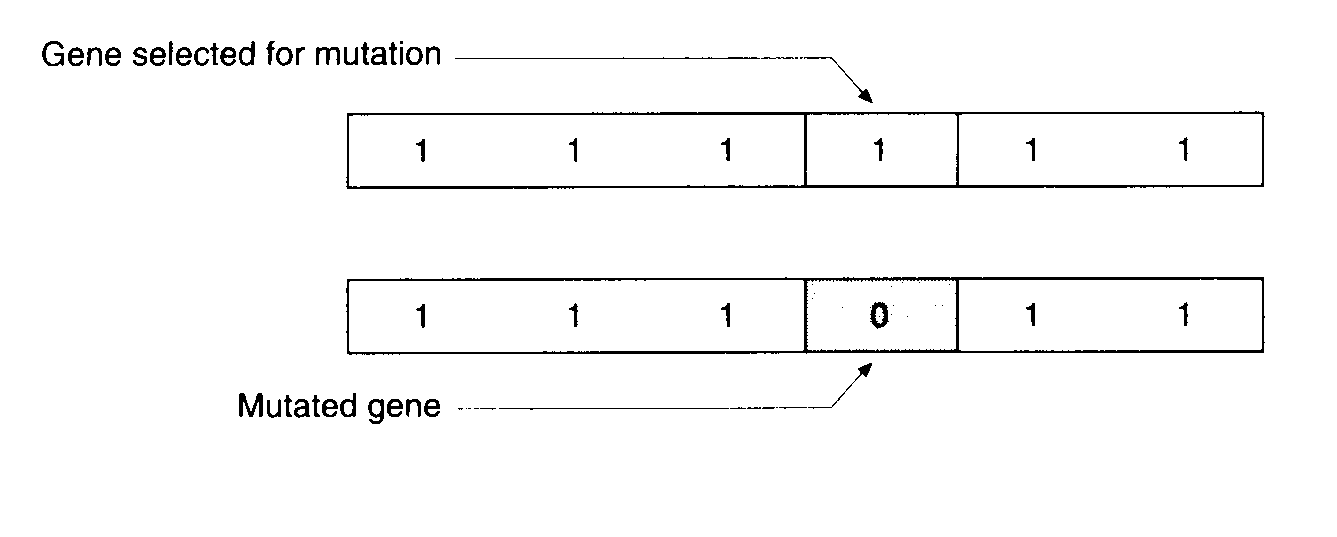
\includegraphics[width=0.4\textheight]{mutation_example.png}
    \end{figure}
	Typically set to be around a few percent
\end{column}
\begin{column}{0.45\textwidth}
\begin{figure}
	\centering
	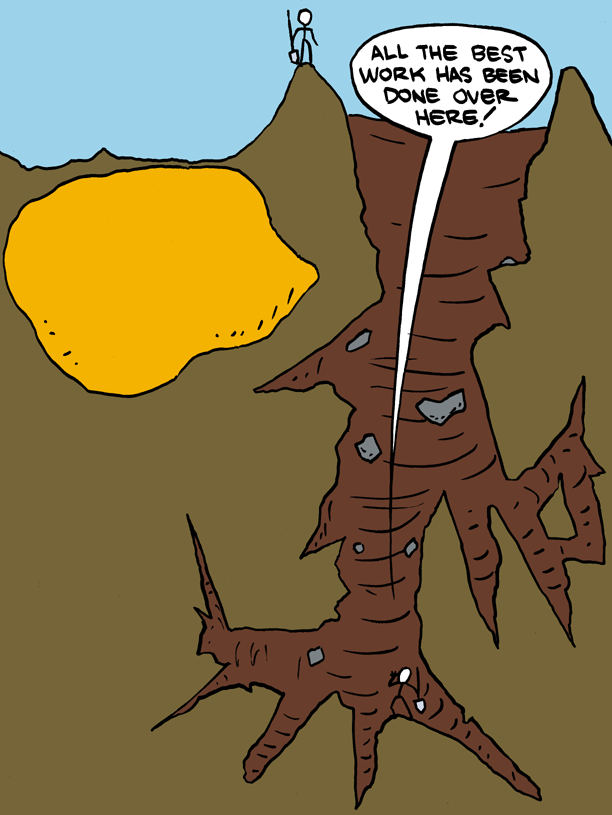
\includegraphics[width=0.75\textwidth]{AllTheBestWork.png}
\end{figure}
\end{column}
\end{columns}
\hyperlink{GAMethod}{\beamerbutton{Return to Optimization}}
\hyperlink{toc}{\beamerbutton{Table of Contents}}
\end{frame}
%%%%%%%%%%%%%%%%%%%%%%%%%%%%%%%%%%%%%%%%%%%%%%%%%%%%%%%%%%%%%%%%%%%%%%%%%%
\begin{frame}{Fitness Function}
The fitness function was chosen to count rate per mass of \iso[6]{Li}, provided that the geometry meet the total count rate criteria.
If it failed to meet the count rate criteria a zero fitness was returned \eqref{eqn:FitnessFun}.
	\tiny
	\begin{align}
			\label{eqn:FitnessFun}
			f(\vec{x})
			= \begin{cases}
			0 & \text{if}~\text{countRate}(\vec{x}) \leq \SI{2.5}{cps\per\nano\gram\iso[252]{Cf}} \\
			\text{countRatePerMass}(\vec{x}) & \text{otherwise}
			\end{cases}
	\end{align}
\begin{columns}[onlytextwidth]
  \begin{column}{0.5\textwidth}
\small
	Computationally intensive to calculate the fitness function 
	\begin{itemize}
		\item Memoization with dictionaries
		\item Multithreading for items not in the dictionary
		\tiny
		\begin{itemize}
			\item This made it sensitive while running
			\item Future work would be to use the PyEvovle multithreading option
		\end{itemize}
	\end{itemize}
	\end{column}
	\begin{column}{0.4\textwidth}
    \begin{figure}
      \centering
      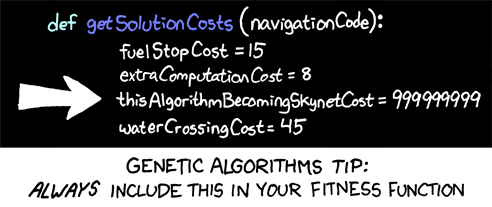
\includegraphics[width=\textwidth]{genetic_algorithms}
    \end{figure}
	\end{column}
\end{columns}
\hyperlink{GAMethod}{\beamerbutton{Return to Optimization}}
\hyperlink{toc}{\beamerbutton{Table of Contents}}
\end{frame}
